\documentclass[10pt]{standalone}
\usepackage{times}
\usepackage{amsmath,amssymb,xspace,xcolor,tikz}
\usetikzlibrary{arrows.meta,positioning,shapes.geometric,calc,fit,backgrounds,decorations.pathmorphing}

\newcommand{\todo}[1]{{\color{red}#1}}
\newcommand{\TODO}[1]{\textbf{\color{red}[TODO: #1]}}
\newcommand{\method}{CxWM\xspace}
\newcommand{\vjepa}{V-JEPA~2.1\xspace}
\newcommand{\flywire}{FlyWire\xspace}
\providecommand{\etal}{\emph{et al}.\xspace}
\providecommand{\ie}{\emph{i.e}.\xspace}
\providecommand{\eg}{\emph{e.g}.\xspace}
\newcommand{\degree}{$^\circ$}
\let\mathpm\pm
\renewcommand{\pm}{\ensuremath{\mathpm}}

% diagram colours (populations match the released 3-D viewer)
\definecolor{cVIS}{RGB}{66,133,244}
\definecolor{cCX}{RGB}{244,160,0}
\definecolor{cMB}{RGB}{52,168,83}
\definecolor{cOUT}{RGB}{219,68,155}
\definecolor{cTeach}{RGB}{90,90,90}
\tikzset{
  box/.style={draw,rounded corners=2pt,minimum height=1.6em,inner sep=4pt,font=\small,align=center},
  pop/.style={box,fill=#1!15,draw=#1!80!black,thick},
  arr/.style={-{Latex[length=2mm]},thick},
  darr/.style={-{Latex[length=2mm]},thick,dashed},
  lbl/.style={font=\scriptsize,align=center},
}
\begin{document}
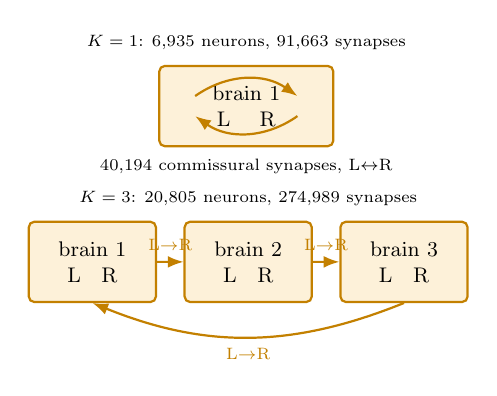
\begin{tikzpicture}[scale=.85,every node/.style={transform shape}]
    \node[pop=cCX,minimum width=2.6cm,minimum height=1.2cm] (b1) {brain 1\\L \quad R};
    \node[lbl,above=1mm of b1] {$K=1$: 6,935 neurons, 91,663 synapses};
    \draw[arr,cCX!80!black] ($(b1.west)+(.55,.15)$) to[bend left=35] ($(b1.east)+(-.55,.15)$);
    \draw[arr,cCX!80!black] ($(b1.east)+(-.55,-.15)$) to[bend left=35] ($(b1.west)+(.55,-.15)$);
    \node[lbl,below=0.5mm of b1] {40,194 commissural synapses, L$\leftrightarrow$R};
    \node[pop=cCX,minimum width=1.9cm,minimum height=1.2cm,below=11mm of b1,xshift=-23mm] (k1) {brain 1\\L \; R};
    \node[pop=cCX,minimum width=1.9cm,minimum height=1.2cm,right=4mm of k1] (k2) {brain 2\\L \; R};
    \node[pop=cCX,minimum width=1.9cm,minimum height=1.2cm,right=4mm of k2] (k3) {brain 3\\L \; R};
    \node[lbl,above=1mm of k2] {$K=3$: 20,805 neurons, 274,989 synapses};
    \draw[arr,cCX!80!black] (k1.east) -- node[lbl,above=1pt]{L$\to$R} (k2.west);
    \draw[arr,cCX!80!black] (k2.east) -- node[lbl,above=1pt]{L$\to$R} (k3.west);
    \draw[arr,cCX!80!black] (k3.south) to[bend left=22] node[lbl,below=1pt]{L$\to$R} (k1.south);
  \end{tikzpicture}
\end{document}
